\section{Entscheidungsbäume}
\begin{figure}
    \centering
    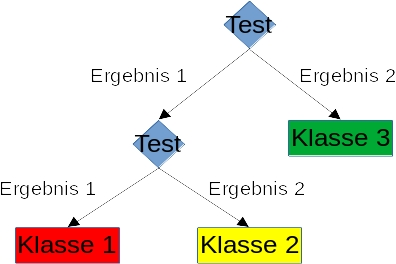
\includegraphics[width=0.5\linewidth]{images/entscheidungsbaum.jpg}
    \caption{Beispiel eines binären Entscheidungsbaums mit 3 möglichen Klassen, die klassifizierbar sind.}
    \label{fig:entscheidungsbaum}
\end{figure}
Der Entscheidungsbaum ist eine rekursive Datenstruktur um Entscheidungsregeln darzustellen. Jedem Blatt ist eine Klasse zugeordnet und allen anderen Knoten ist ein \textit{Test} zugeordnet. Der Test hat eine Reihe von sich
gegenseitig auschließenden Ergebnissen. Die Zuordnung einer Klasse zu einem Objekt wird durch das Traversieren dieses Baumes bestimmt bis ein Blatt erreicht wird \cite{quinlan1990decision}. Abbildung \ref{fig:entscheidungsbaum}
zeigt einen Entscheidungsbaum, wo jeder Test zwei mögliche Ergbnisse hat, i. e. einen binären Entscheidungsbaum. Möglich wäre aber auch das jeder Test eine arbiträre Anzahl an möglichen Ergebnissen hätte.

\subsection{Konstruktion}
\label{sec:construction}
Es gibt viele verschiedene Algorithmen um Entscheidungsbäume zu erzeugen: \texttt{ID3}, \texttt{C4.5}, \texttt{C5}, \texttt{CART}, \texttt{CHAID}, \texttt{QUEST},
\texttt{GUIDE}, \texttt{CRUISE} and \texttt{CTREE}. Am häufigsten wird ID3 (Iterative Dichotomizer 3), bzw. C4.5, welches eine Weiterentwicklung von ID3 ist, und CART (Classification and Regression Trees) verwendet \cite{scikit-learn, singh2014comparative}.
Diese Arbeit verwendet die Implementierung für Entscheidungsbaumklassifizierer von \textit{Scikit-Learn}, die eine optimierte Version von CART nutzt \cite{ScikitLearnCART}. Scikit-Learn ist ein Python-Modul, das eine
große Auswahl von Algorithmen zum maschinellen Lernen implementiert \cite{scikit-learn}.

\subsubsection{CART: Classification and Regression Trees}
Die Konstruktion eines optimalen binären Entscheidungsbaum ist NP-Komplett \cite{laurent1976constructing}. CART ist ein Greedy-Algorithmus, der lokal immer die beste Teilung wählt.
\begin{lstlisting}[label=lst:CARTtreeGrowing,caption={Skizze von vereinfachten Baumwachstumsalgorithmus \cite{steinbergCART}.}]
    Weise dem Wurzelknoten alle Trainingsdaten zu.
    Definiere den Wurzelknoten als Blatt.
    WHILE True:
        Neue_Teilungen = 0
        FOR jedes Blatt:
            IF die Größe der zugewiesenen Trainingsdaten zu klein ist oder alle Einträge der Trainingsdaten zur gleichen Klasse gehören:
                CONTINUE
            Finde das Attribut, das am besten den Knoten in zwei Kindesknoten unterteilt mit einer erlaubten Teilungsregel.
            Neue_Teilungen += 1
        IF Neue_Teilungen == 0:
            break
\end{lstlisting}
Listing \ref{lst:CARTtreeGrowing} skizziert wie CART initial einen maximal großen Baum generiert indem die Trainingsdaten solange geteilt werden bis keine weitere Teilung mehr möglich ist oder alle Einträge der gleichen
Klasse zugeordnet sind. Zuletzt beginnt der Reduzierungsprozess indem Teilbäume gelöscht werden, die die Klassifizierungsgenauigkeit nicht erhöhen oder der Zuwachs unter einem Nutzer definierten
Schwellenwert liegt \cite{steinbergCART}.